% Kapitel 2 - Grafik und diverses
\chapter{Grafik und Diverses}
\section{Grafiken einbinden}

% normal
\subsection{Standard}
\begin{figure}[!htbp]
			\begin{center}
				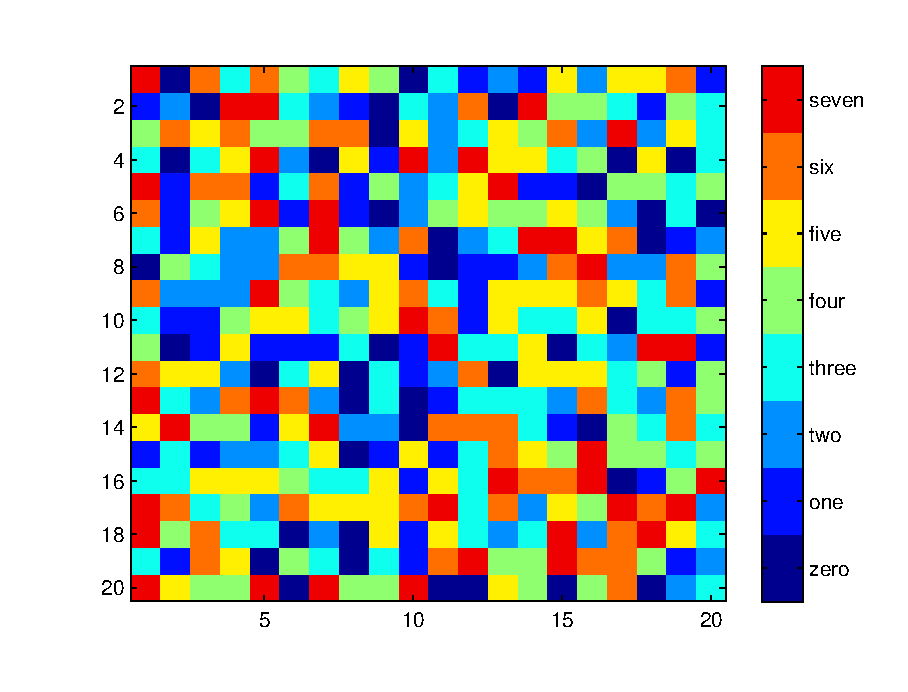
\includegraphics[scale = .9]{colorbar}
				\caption{Colorbar}
				\label{kap3:colorbar}
  		\end{center}
\end{figure}

% nebeneinander
\subsection{nebeneinder}
So lassen sich Bilder nebeneinander darstellen.
	\begin{figure}[!htbp]
		% TU Logo
  	\begin{minipage}{0.4\linewidth}
			\begin{center}
				\includegraphics[scale=1]{tu-logo.eps}
  		\end{center}
  	\end{minipage}
		\hfill
		% EMSP Logo
  	\begin{minipage}{0.45\linewidth}
  		\begin{center}
				\includegraphics[scale=0.3]{Logo_final.eps}
  		\end{center}
  	\end{minipage}
  	\caption{zwei Grafiken}
  	\label{kap3:neben}
	\end{figure}

\section{Diverses}
\subsection{Literaturverweise}

Einbinden von Verweisen: \cite{brig96}
Sieht im Text dann einfach wie \cite{Kamm02} aus.

\subsection{Verweise innerhalb des Dokuments}
Beispiele f�r Formeln gibt es in \ref{sec:formeln}

\subsection{Tabellen}

Beispiel f�r tabular-Umgebung

\begin{table}[!ht]
\caption[In Matlab]{Matlab-Befehle}
\label{tab:ML1}
\begin{tabular}{|| p{7cm} | p{6cm} ||} \hline\hline
I=eye(N);      																									& Einheitsmatrix \\ \hline
e=zeros(N,1); e(j)=1; 																					& Einheitsvektor\\ \hline
D=diag([d11,d22,...,dNN]); 																			& Diagonalmatrix \\ \hline
J=rot90(eye(N)); 																								& Koidentit�tsmatrix \\ \hline
E=ones(M,N); 																										& Einsmatrix \\ \hline
eins=ones(N,1); 																								& Einsvektor \\ \hline
t1=[t11,t12,...,t1N]; t2=[t11,t21,...,tN1]; 										& \\
T=toeplitz(t1,t2);  																						& Toeplitzmatrix \\ \hline
t=[t11,t12,...,t1N]; T=toeplitz(t); 														& symmetrische Toeplitzmatrix \\ \hline
x=[x1,x2,...,xN]; v=rot90(vander(x))'; 													& Vandermonde-Matrix \\ \hline
L=tril(A); 																											& untere Dreiecksmatrix der Matrix A \\ \hline
U=triu(A); 																											& obere Dreiecksmatrix der Matrix A \\ \hline\hline
\end{tabular}
\end{table}

\vspace*{2cm}

Das ganze nun mit longtable und hhline, aber ohne Beschriftung

\begin{longtable}{|| p{7cm} | p{6cm} ||} \hhline{||=|=||}
I=eye(N);       																								& {Einheitsmatrix} \\\hline
e=zeros(N,1); e(j)=1; 																					& Einheitsvektor\\ \hline
D=diag([d11,d22,...,dNN]); 																			& Diagonalmatrix \\ \hline
J=rot90(eye(N)); 																								& Koidentit�tsmatrix \\ \hline
E=ones(M,N); 																										& Einsmatrix \\ \hline
eins=ones(N,1); 																								& Einsvektor \\ \hline
t1=[t11,t12,...,t1N]; t2=[t11,t21,...,tN1]; 										& \\
T=toeplitz(t1,t2);  																						& Toeplitzmatrix \\ \hline
t=[t11,t12,...,t1N]; T=toeplitz(t); 														& symmetrische Toeplitzmatrix \\ \hline
x=[x1,x2,...,xN]; v=rot90(vander(x))'; 													& Vandermonde-Matrix \\ \hline
L=tril(A); 																											& untere Dreiecksmatrix der Matrix A \\ \hline
U=triu(A); 																											& obere Dreiecksmatrix der Matrix A \\ \hline\hline
\end{longtable}